
\begin{frame}
  \frametitle{Probability Distributions}
  Here, we change the meaning of the variables to represent probability
  distributions.  $C$ is a constant given by
  the marginal likelihood, which can be ignored when calculating relative
  probabilities, and $\boldsymbol{d}$ and $\boldsymbol{m}$ represent the training
  data set and model parameters, respectively. Thus,
  $P(\boldsymbol{d}|\boldsymbol{m})$ is the likelihood distribution function,
  $P(\boldsymbol{m})$ is the prior probability distribution, and
  $P(\boldsymbol{m}|\boldsymbol{d})$ is the posterior probability distribution.
  \begin{equation}
    P(\boldsymbol{m}|\boldsymbol{d}) = C\ *\
    P(\boldsymbol{d}|\boldsymbol{m})\ *\ P(\boldsymbol{m})
  \end{equation}
 
  Mathematically speaking, the distributions are obtained by integrating over the
  relevant probability densities.  For example, the prior probability
  distribution can be calculated, where
  $\boldsymbol{m}$ is the range of predicted model parameters, i.e. burnup
  values, and $\boldsymbol{d}$ is a set of nuclide vectors. Also, here,
  $\rho(\boldsymbol{x}) = \prod_{i} \rho(x_i)$. 
  \begin{equation}
    P(\boldsymbol{m}) = \int_{\boldsymbol{m}} \rho(\boldsymbol{d}) d\boldsymbol{d}
  \end{equation}
  Similarly, the likelihood distribution function is obtained as in Equation 
  \begin{equation}
    P(\boldsymbol{d}|\boldsymbol{m}) = \int_{\boldsymbol{d}, \boldsymbol{m}} \rho(\boldsymbol{d}|\boldsymbol{m}) d\boldsymbol{m}
  \end{equation}
  In practice, however, these density functions are not calculated directly.
  Below, the methods chosen to estimate the functions in this work are addressed.
\end{frame}

\begin{frame}
  \frametitle{Estimating Density Functions}
  Convert wordage to graphic?
\end{frame}

\begin{frame}
  \frametitle{Posterior Odds}
  \begin{equation}
    \frac{P(m_i|d)}{P(m_j|d)} = B_{ij} \frac{P(m_i)}{P(m_j)}
  \end{equation}
  \begin{table}
    \centering
    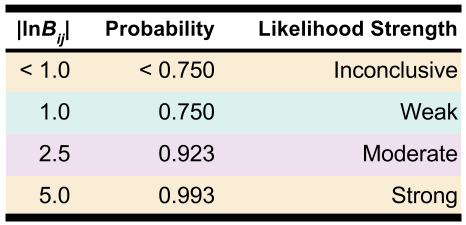
\includegraphics[width=0.7\linewidth]{./figures/evidence-strength.png}
    \caption{Model comparison using likelihood strength}
  \end{table}
\end{frame}
